% -*- Mode: latex; -*-
% $HeadURL: https://outreach.scidac.gov/svn/hpctoolkit/trunk/doc/manual/hpcviewer.tex $
% $Id: hpcviewer.tex 3336 2011-01-03 23:29:25Z tallent $


% ----------------------------------------------------------
% traceviewer
% ----------------------------------------------------------

\newcommand{\crosshair}{crosshair}
\newcommand{\traceview}{Trace view}
\newcommand{\depthview}{Depth view}
\newcommand{\summaryview}{Summary view}
\newcommand{\miniview}{Mini map view}
\newcommand{\callview}{Call path view}


% ===========================================================================
% ===========================================================================

\section{\hpctraceviewer{} overview}

\begin{figure}[t]
\centering{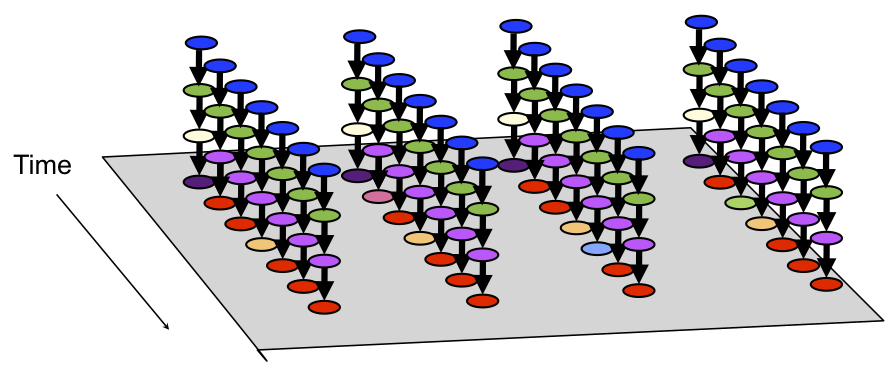
\includegraphics[width=\textwidth]{fig/hpctraceviewer-callpath.png}}
\caption{Logical view of trace call path samples on three dimensions: time, process rank and call path depth.}
\label{fig:hpctraceviewer-callpath}
\end{figure}

\HPCToolkit{} provides two applications to visualize performance data: \hpcviewer{}~\cite{Adhianto-MC-Ta:2010:PSTI-hpcviewer} for performance profile presentation tool, and \hpctraceviewer{}~\cite{Tallent-MC-etal:2011:ICS-hpctoolkit-scalable-tracing} of performance presentation tool for interactive examination of performance-trace databases.
Here, we describe \hpctraceviewer{} which interactively presents a large-scale trace without concern for the scale of parallelism it represents.

In order to generate a trace data, the user has to run \hpcrun{} with {\tt -t } flag to enable the tracing. It is preferable to sample with regular time-based events like {\tt WALLCLOCK} or {\tt PAPI\_TOT\_CYC} instead of irregular time-based events such as {\tt PAPI\_FP\_OPS} and {\tt PAPI\_L3\_DCM}.

As shown in Figure~\ref{fig:hpctraceviewer-callpath}, trace call path data generated by \hpcprof{} comprises samples from three dimensions: \emph{process rank} (or thread rank if the application is multithreaded), \emph{time} and \emph{call path} depth.
Therefore, a \emph{\crosshair} in \hpctraceviewer{} is defined by a triplet $(p,t,d)$ where $p$ is the selected process rank, $t$ is the selected time, and $d$ is the selected call path depth. 

\hpctraceviewer{} visualizes the samples for process and time dimension with \emph{\traceview} (Section~\ref{sec:traceview}), call path depth and time dimension with \emph{\depthview} (Section~\ref{sec:depthview}) and a call path of a specific process and time with \emph{\callview} (Section~\ref{sec:callview}).
Each view has its own use to pinpoint performance problem which will be described in the next sections.

In \hpctraceviewer, each procedure is assigned specific color based on labeled nodes in \hpcviewer. Figure~\ref{fig:hpctraceviewer-callpath} shows that the top level (level 1) in the call path is assigned the same color: blue, which is the main entry program in all process and all time.
The next depth (level 2), all processes have the same node color, i.e. green, which is another procedure. 
In the following depth (level 3), all processes in the first time step have light yellow node and on the time steps, they have purple. This means that in the same depth and time, not all processes are in the same procedure.
This color assignment is important to visually identify load imbalance in a program.

% ===========================================================================
% ===========================================================================

\section{Launching}

\hpctraceviewer{} can either be launched from a command line (Linux/Unix platform) or by clicking the \hpctraceviewer{} icon (for Windows, Mac OS X and Linux/Unix platform).
The command line syntax is as follows:
\begin{quote}
\begin{verbatim}
  hpctraceviewer [options] [<hpctoolkit-database>]
\end{verbatim}
\end{quote}
Here, \texttt{<hpctoolkit-database>} is an optional argument to load a database automatically.
Without this argument, \hpctraceviewer{} will prompt for the location of a database.

The possible options are as follows:
\begin{itemize}

 \item \texttt{-consolelog}: Send log entries to a console in addition to a log file.
   (To get a console window, be sure to use java as the VM instead of javaw.)

 \item \texttt{-debug}: Log additional information about plug-in dependency problems.
\end{itemize}


% ===========================================================================
% ===========================================================================

\section{Views}

\begin{figure}[t]
\centering{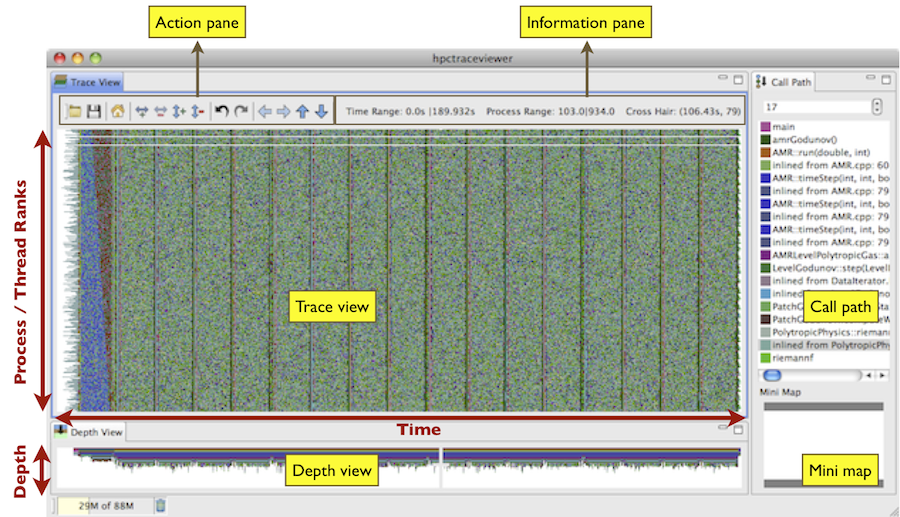
\includegraphics[width=\textwidth]{fig/hpctraceviewer-legend.png}}
\caption{An annotated screenshot of \hpctraceviewer{}'s interface.}
\label{fig:hpctraceviewer-legend}
\end{figure}

Figure~\ref{fig:hpctraceviewer-legend} shows an annotated screenshot of \hpctraceviewer{}'s user interface presenting a call path profile.
The annotations highlight \hpctraceviewer{}'s four principal window panes: \traceview, \depthview, \callview{} and \miniview.

\begin{itemize}
\item \textbf{\traceview} (left, top):
  This is \hpctraceviewer{}'s primary view.
  This view, which is similar to a conventional process/time (or space/time) view, shows time on the horizontal axis and process (or thread) rank on the vertical axis; time moves from left to right.
  Compared to typical process/time views, there is one key difference.
  To show call path hierarchy, the view is actually a user-controllable slice of the process/time/call-path space.
  Given a call path depth, the view shows the color of the currently active procedure at a given time and process rank.
  (If the requested depth is deeper than a particular call path, then \hpctraceviewer{} simply displays the deepest procedure frame and, space permitting, overlays an annotation indicating the fact that this frame represents a shallower depth.)

  \hpctraceviewer{} assigns colors to procedures based on (static) source code procedures.
  Although the color assignment is currently random, it is consistent across the different views.
  Thus, the same color within the Trace and Depth Views refers to the same procedure.

  The Trace View has a white \crosshair{} that represents a selected point in time and process space.
  For this selected point, the Call Path View shows the corresponding call path.
  The Depth View shows the selected process.

\item \textbf{\depthview} (left, bottom):
  This is a call-path/time view for the process rank selected by the \traceview's \crosshair{}.
  Given a process rank, the view shows for each virtual time along the horizontal axis a stylized call path along the vertical axis, where `main' is at the top and leaves (samples) are at the bottom.
  In other words, this view shows for the whole time range, in qualitative fashion, what the Call Path View shows for a selected point.
  The horizontal time axis is exactly aligned with the Trace View's time axis; and the colors are consistent across both views.
  This view has its own \crosshair{} that corresponds to the currently selected time and call path depth.

\item \textbf{\summaryview} (left, bottom):
  The view shows for the whole time range dislayed, the proportion of each subroutine in a certain time.
  Similar to Depth view, the time range in Summary reflects to the time range in the Trace view. 

\item \textbf{\callview} (right, top):
  This view shows two things: (1) the current call path depth that defines the hierarchical slice shown in the Trace View; and (2) the actual call path for the point selected by the Trace View's \crosshair{}.
  (To easily coordinate the call path depth value with the call path, the Call Path View currently suppresses details such as loop structure and call sites; we may use indentation or other techniques to display this in the future.)

\item \textbf{\miniview} (right, bottom):
  The Mini Map shows, relative to the process/time dimensions, the portion of the execution shown by the Trace View.
  The Mini Map enables one to zoom and to move from one close-up to another quickly.

\end{itemize}

% ===========================================================================
% ===========================================================================

\subsection{\traceview}
\label{sec:traceview}

\traceview{} is divided into two parts: the top part which contains \emph{action pane} and the \emph{information pane}, and the main view which displays the traces. 

The buttons in the action pane are the following:
\begin{itemize}

\item \textbf{Home} 
\includegraphics[scale=.5]{fig/hpctraceviewer-button-home-screen.png} : Resetting the view configuration into the original view, i.e., viewing traces for all times and processes.
\item \textbf{Horiontal zoom in 
\includegraphics{fig/hpctraceviewer-button-zoom-in-time.png} / out }
\includegraphics{fig/hpctraceviewer-button-zoom-out-time.png} : Zooming in/out the time dimension of the traces. 
\item \textbf{Vertical zoom in 
\includegraphics[scale=.5]{fig/hpctraceviewer-button-zoom-in-process.png} / out 
\includegraphics[scale=.5]{fig/hpctraceviewer-button-zoom-out-process.png} }: Zooming in/out the process dimension of the traces.
\item \textbf{Navigation buttons} 
\includegraphics[scale=.5]{fig/hpctraceviewer-button-go-east.png}, 
\includegraphics[scale=.5]{fig/hpctraceviewer-button-go-west.png}, 
\includegraphics[scale=.5]{fig/hpctraceviewer-button-go-north.png}, 
\includegraphics[scale=.5]{fig/hpctraceviewer-button-go-south.png} : Navigating the trace view to the left, right, up and bottom, respectively. It is also possible to navigate with the arrow keys in the keyboard. Since \traceview{} does not support scrool bars, the only way to navigate is through navigation buttons (or arrow keys).
\item \textbf{Undo} 
\includegraphics[scale=.5]{fig/hpctraceviewer-button-undo.png} : Canceling the action of zoom or navigation and returning back to the previous view configuration.
\item \textbf{Redo} 
\includegraphics[scale=.5]{fig/hpctraceviewer-button-redo.png} : Redoing of previously undo change of view configuration.
\item \textbf{Save} 
\includegraphics[scale=.5]{fig/hpctraceviewer-button-save.png}  / \textbf{Open 
\includegraphics[scale=.7]{fig/hpctraceviewer-button-open.png} a view configuration} : Saving/loading a saved view configuration. 
A view configuration file contains the information of the current dimension of time and process, the depth and the position of the \crosshair{}. 
It is recommended to store the view configuration file in the same directory as the database to ensure that the view configuration file matches well with the database since the file does not store which database it is associated with. 
Although it is possible to open a view configuration file which is associated from different database, it is highly not recommended since each database has different time/process dimensions and depth.


\end{itemize}

The information pane contains some information concerning the range status of the current displayed data.
\begin{itemize}
 \item \textbf{Time Range}. The information of current time-range (horizontal) dimension. 
 \item \textbf{Process Range}. The information of current process-range (vertical) dimension. The ranks are formatted in the following notation:
\begin{verbatim}
  <process_id> . <thread_id>
\end{verbatim}
Hence, if the ranks are 0.0, 0.1, \dots{} 31.0, 31.1 it means MPI process 0 has two threads: thread 0 and thread 1 (similarly with MPI process 31). 

 \item \textbf{Cross Hair}. The information of current \crosshair{} position in time and process dimensions. 
\end{itemize}

% ===========================================================================
% ===========================================================================
\subsection{\depthview}
\label{sec:depthview}

\depthview{} shows all the call path for a certain time range $[t_1,t_2]= \{t | t_1\leq t\leq t_2\}$ in a specified process rank $p$. The content of \depthview{} is always consistent with the position of the \crosshair{} in \traceview{}.
For instance once the user clicks in process $p$ and time $t$, while the current depth of call path is $d$, then the \depthview's content is updated to display all the call path of process $p$ and shows its \crosshair{} on the time $t$ and the call path depth $d$.

On the other hand, any user action such as \crosshair{} and time range selection in \depthview{} will update the content within \traceview. Similarly, the selection of new call path depth in \callview{} invokes a new position in \depthview.

In \depthview{} a user can specify a new \crosshair{} time and a new time range.
\paragraph{Specifying a new \crosshair{} time.} Selecting a new \crosshair{} time $t$ can be performed by clicking a pixel within \depthview{}. This will update the \crosshair{} in \traceview{} and the call path in \callview.

\paragraph{Selecting a new time range.} Selecting a new time range $[t_m,t_n]= \{t | t_m\leq t\leq t_n\}$ is performed by first clicking the position of $t_m$ and drag the cursor to the position of $t_n$. A new content in \depthview{} and \traceview{} is then updated. Note that this action will not update the call path in \callview{} since it does not change the position of the \crosshair.


% ===========================================================================
% ===========================================================================
\subsection{\summaryview}
\label{sec:summaryview}

\summaryview{} presents the proportion of number of calls of time $t$ across the current displayed rank of proces $p$. 
Similar to \depthview, the time range in \summaryview{} is always consistent with the time range in \traceview{}.


% ===========================================================================
% ===========================================================================
\subsection{\callview}
\label{sec:callview}

\begin{figure}[t]
\centering{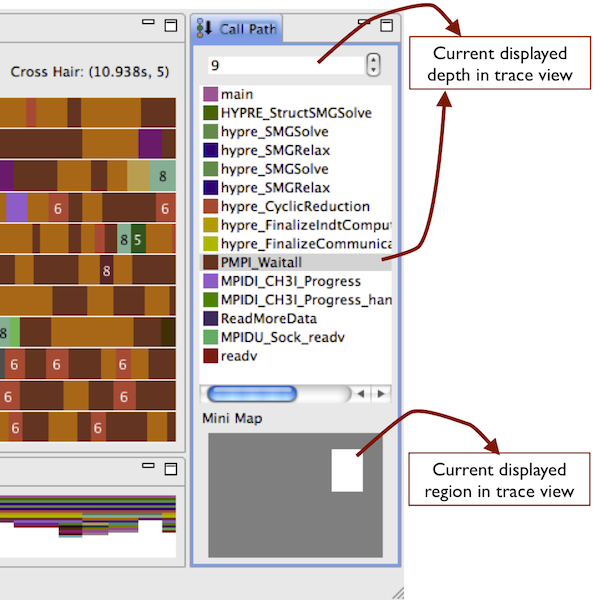
\includegraphics{fig/hpctraceviewer-callpath-legend.png}}
\caption{An annotated screenshot of \hpctraceviewer{}'s \callview.}
\label{fig:hpctraceviewer-callpath-legend}
\end{figure}

This view lists the call path of process $p$ and time $t$ specified in \traceview{} and \depthview.
Figure~\ref{fig:hpctraceviewer-callpath-legend} shows a call path from depth $0$ to depth $14$, and the current depth is $9$ as shown in the depth editor (located on the top part of the view).

In this view, the user can select the depth dimension of \traceview{} by either typing the depth in the depth editor or selecting a procedure in the table of call path.

% ===========================================================================
% ===========================================================================
\subsection{\miniview}
\label{sec:miniview}

The \miniview{} shows, relative to the process/time dimensions, the portion of the execution shown by the \traceview.
In \miniview{}, the user can select a new process/time $(p_a,t_a),(p_b,t_b)$ dimensions by clicking the first process/time position $(p_a,t_a)$ and then drag the cursor to the second position $(p_b,t_b)$.
The user can also moving the current selected region to another region by clicking the white rectangle and drag it to the new place.


% ===========================================================================
% ===========================================================================

\begin{figure}[t]
\centering{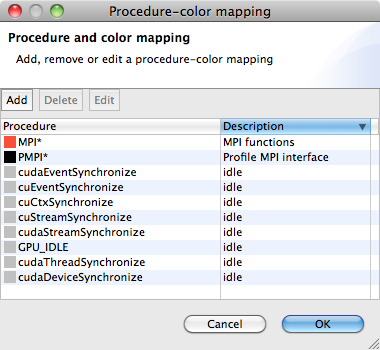
\includegraphics[width=3.4in]{fig/hpctraceviewer-dialog-mapping}}
\caption{Procedure-color mapping dialog box. This window shows that any procedure names that match with "MPI*" pattern are assigned with red, while procedures that match with "PMPI*" pattern are assigned with color black.}
\label{fig:hpctraceviewer-mapping}
\end{figure}

\begin{figure}[t]
\centering{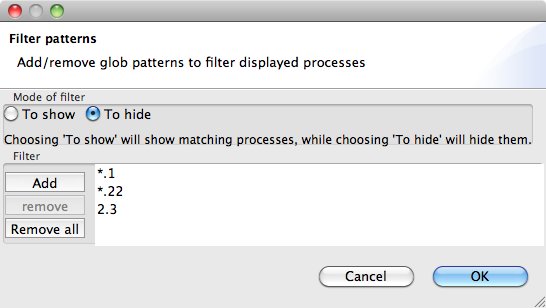
\includegraphics[width=4in]{fig/hpctraceviewer-dialog-filter.png}}
\caption{Rank filter dialog box. This window shows that all rank IDs that match with the list of patterns will be hidden from the display. For example, ranks 1.1, 2.1, 1.22, 1.3 will be hidden.}
\label{fig:hpctraceviewer-filter}
\end{figure}


\section{Menus}
\hpctraceviewer{} provides three main menus:
\begin{itemize}
 \item \textbf{File} menu which contains two sub menus:
 \begin{itemize}
   \item \textbf{Open database}: to load a database experiment directory. The directory has to contain \texttt{experiment.xml} (CCT and metric information) or \texttt{callpath.xml} (uniquely CCT information), and \texttt{*.hpctrace} or \texttt{experiment.mt} files which provide trace information.
   \item \textbf{Exit}: to quit the application.
 \end{itemize}
 \item \textbf{View} menu to enhance appearance which contains two sub menus:
 \begin{itemize}
   \item \textbf{Show debug info}: to enable/disabe the display of debugging information in the form of `$a(b)$' where $a$ is the maximum depth (this number is shown if the current depth reaches the maximum depth) and $b$ is the number of records on the trace view. 
The number of records can be useful to identify blocking procedures (such as I/O operations). Note: the numbers are displayed only if there's enough space in the process time line.
   \item \textbf{Using midpoint painting}: if checked, the trace painting will use \emph{midpoint} painting algorithm. By using the later, for every samples $S_1$ at time $T_1$, $S_2$ at time $T_2$ and $S_3$ at time $T_3$, \hpctraceviewer{} renders a block from $T_1$ to $\frac{T1+T2}{2}$ to sample $S_1$, and a block from from  $\frac{T1+T2}{2}$ to  $\frac{T2+T3}{2}$ for sample $S_2$, and so forth. 
If the menu is not checked, then a simpler \emph{rightmost} algorithm is used: it will render a block from  $T_1$ to $T_2$ for sample $S_1$, and a block from $T_2$ to  $T3$ for sample $S_2$, and so forth.
   \item \textbf{Show procedure-color mapping}: to open a window which shows customized mapping between a procedure pattern and a color (Figure~\ref{fig:hpctraceviewer-mapping}). \hpctraceviewer{} allows users to customize assignment of a pattern of procedure names with a specific color.
   \item \textbf{Filter ranks}: to open a window for selecting which ranks should be displayed (Figure~\ref{fig:hpctraceviewer-filter}). Recall that a rank can be a process (e.g. MPI applications), a thread (OpenMP applications) or both (hybrid MPI and OpenMP applications). \hpctraceviewer{} allows two types of filtering: either you specify which ranks \textit{to show} or \textit{to hide} (default is to hide). 
To add a pattern to filter, you need to click "add" button and type the pattern in the dialog box. To remove a pattern, you have to select the pattern to remove, and click "Remove" button. Finally, clicking to "Remove all" button will clear the list of patterns.
 \end{itemize}
 \item \textbf{Window} menu to manage the layout of the application. The menu only provide one sub menu:
 \begin{itemize}
  \item \textbf{Reset layout}: to reset the layout to the original one.
 \end{itemize}
\end{itemize}

\hpctraceviewer{} also provides a context menu to save the current image of the view. 
This context menu is available is three views: trace view, depth view and summary view.

% ===========================================================================
% ===========================================================================



\section{Limitations}

Some important \hpctraceviewer{} limitations are listed below:
\begin{itemize}

\item \textbf{Handling hybrid MPI and OpenMP applications are not fully supported}.
	Although it is possible to display trace data from mixed programming models such as MPI and OpenMP, the callpath between threads and processes are not fully consistent; thus it may confuse the user. Note: some MPI runtime spawns helper-threads which makes the trace appears to have more threads than it should be.

\item \textbf{No image print}.
	At the moment \hpctraceviewer{} does not support saving and printing images of the traces.

\item \textbf{Not scalable on IBM Power7 and BGQ platforms for large database}.
	Displaying a large database (more than 2 GB of \texttt{experiment.mt} file on IBM Power7 and BGQ is very slow. This is a known issue, and we are working on this.


\end{itemize}
